\section{Evaluation}
\label{sec:eval}
\begin{figure*}[t]
    \centering
    \begin{subfigure}[b]{0.32\textwidth}
        \centering
        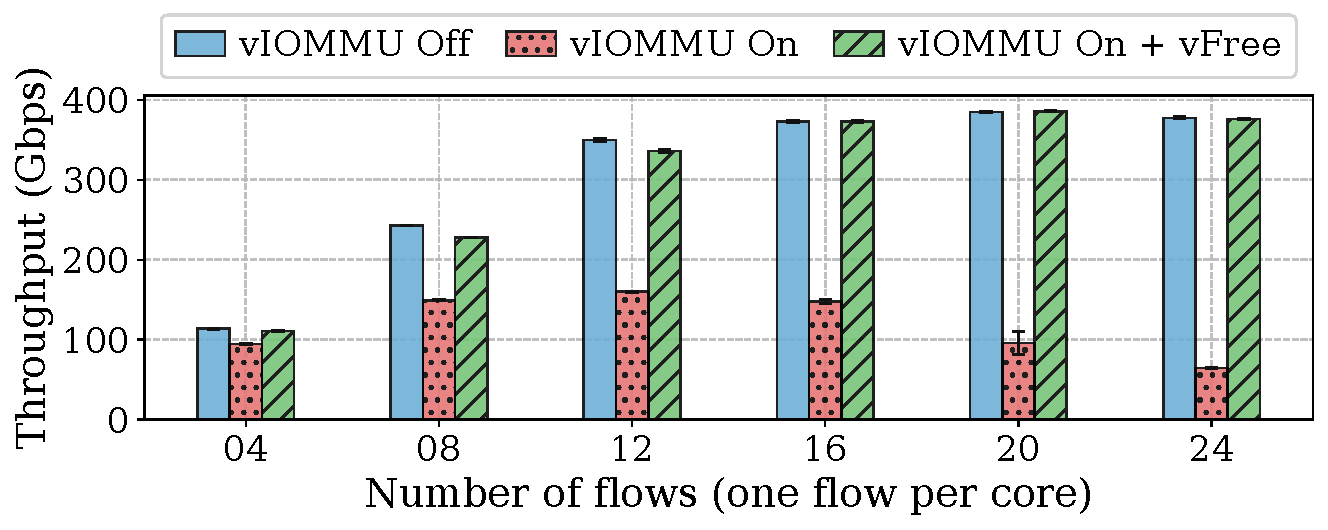
\includegraphics[width=\textwidth]{figures/eval_core_exp-tput.pdf}
        \caption{Throughput}
        \label{fig:eval-core-tput}
    \end{subfigure}
    \hfill
    \begin{subfigure}[b]{0.32\textwidth}
        \centering
        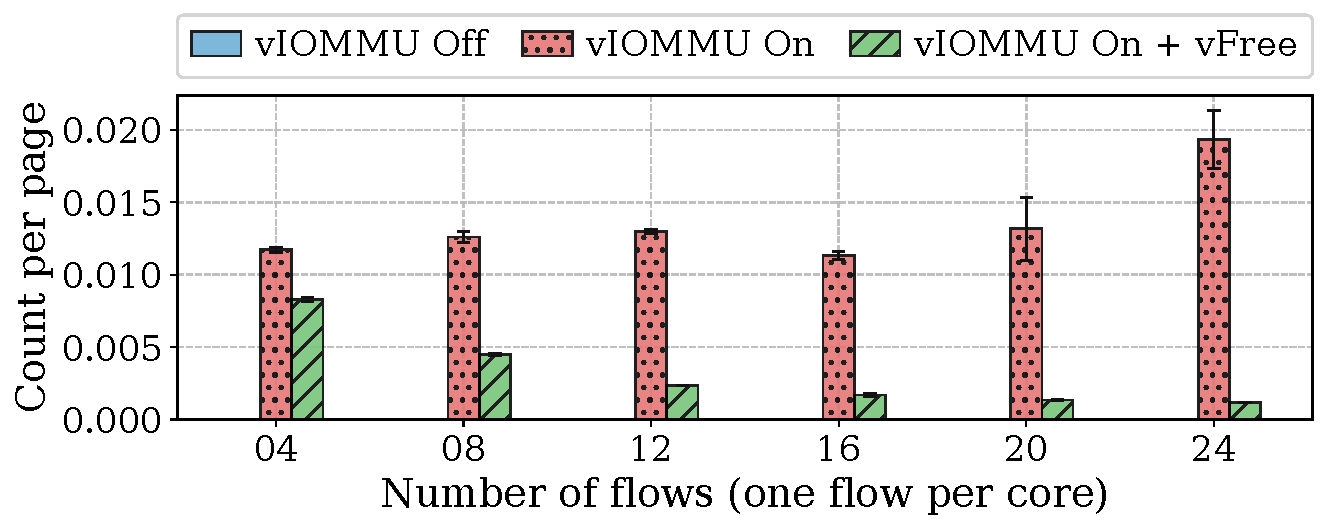
\includegraphics[width=\textwidth]{figures/eval_core_exp-qi_submit_sync-count_per_page.pdf}
        \caption{IOTLB invalidation count per page}
        \label{fig:eval-core-qi}
    \end{subfigure}
    \hfill
    \begin{subfigure}[b]{0.32\textwidth}
        \centering
        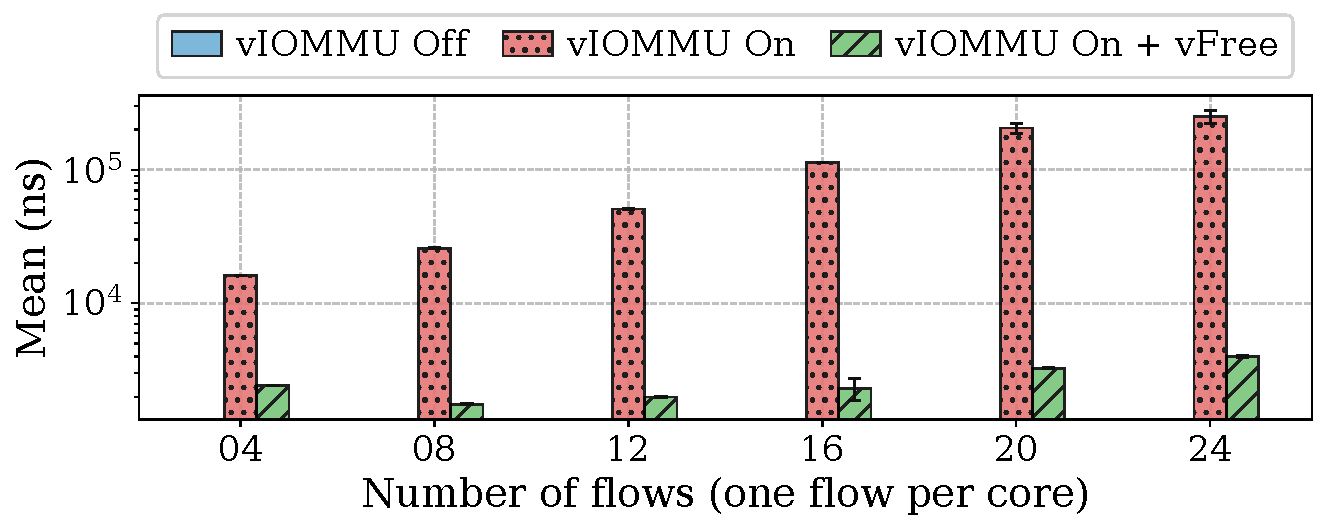
\includegraphics[width=\textwidth]{figures/eval_core_exp-cache_tag_flush_range-mean_ns.pdf}
        \caption{Average time for IOTLB invalidation}
        \label{fig:eval-core-flush}
    \end{subfigure}
    \caption{Performance of vIOMMU off, vanilla vIOMMU on nested translation, and vIOMMU + \brand with Rx traffic.
    Experiments run with different number of cores with one flow per core. 
    }
    \label{fig:eval-core}
\end{figure*}

\begin{figure*}[t]
    \centering
    \begin{subfigure}[b]{0.32\textwidth}
        \centering
        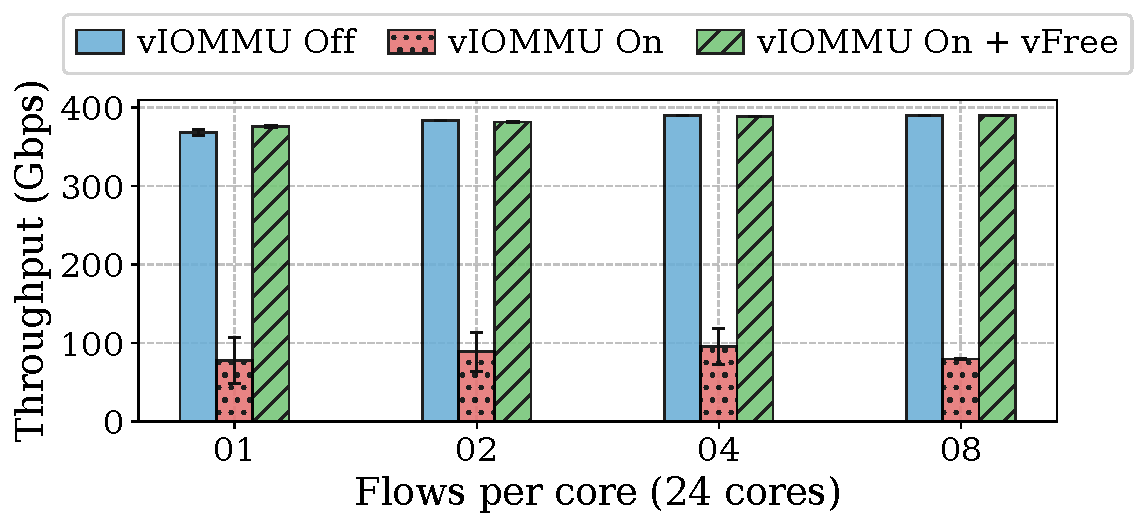
\includegraphics[width=\textwidth]{figures/stress_exp-tput.pdf}
        \caption{Throughput}
        \label{fig:stress-tput}
    \end{subfigure}
    \hfill
    \begin{subfigure}[b]{0.32\textwidth}
        \centering
        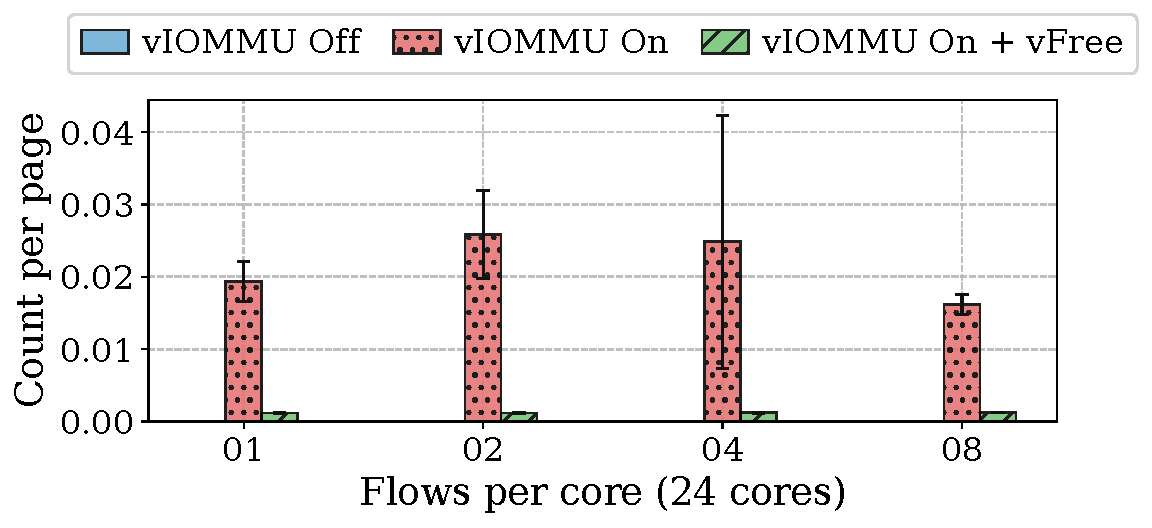
\includegraphics[width=\textwidth]{figures/stress_exp-qi_submit_sync-count_per_page.pdf}
        \caption{IOTLB invalidation count per page}
        \label{fig:stress-qi}
    \end{subfigure}
    \hfill
    \begin{subfigure}[b]{0.32\textwidth}
        \centering
        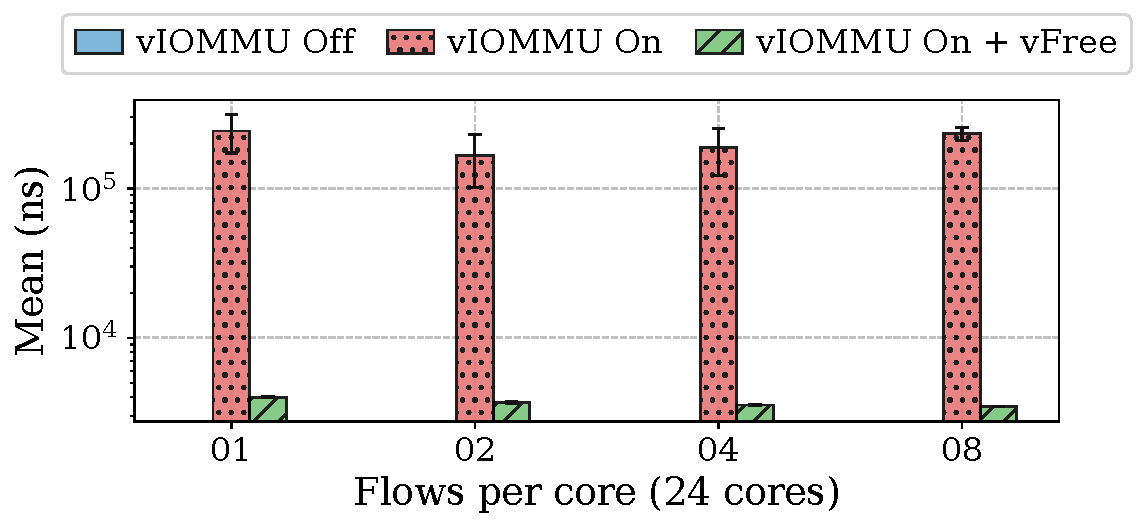
\includegraphics[width=\textwidth]{figures/stress_exp-cache_tag_flush_range-mean_ns.pdf}
        \caption{Average time for IOTLB invalidation}
        \label{fig:stress-flush}
    \end{subfigure} 
    \caption{Performance of vIOMMU off, vanilla vIOMMU on nested translation, and vIOMMU + \brand with Rx traffic.
    Experiments run with different number of flows with 24 cores. 
    }
    \label{fig:stress}
\end{figure*}



\name\ is guest OS-only solution. We implemented on top of Linux 6.12.9.
By default, we built async invalidation with distributed-leader-follower scheme with maximum flushes of 1.
We focus on four research questions:

\begin{enumerate}
    \item How much benefit does \brand provide for real-world applications?
    \item How does \brand perform under various high-performance networking setups?
    \item How does each component of \brand contribute to its performance?
    \item What are the resource overheads of \brand, and how sensitive is its performance to varying system configurations and memory constraints?
    \item Multi-VM. 
\end{enumerate}



\subsection{Evaluation Setup}

We setup the evaluation framework mimicking production system.
We setup two Emerald Rapids machines as server and client. Both of them support nested IOMMU.
The two machines come with Intel Xeon Platinum 8592V CPU.
The server machine has four NUMA nodes, and the client machine has two NUMA nodes.
All NUMA nodes are attached with 32 CPU cores and 252 GB of memory.
The machines have Mellanox ConnectX-7 NIC directly connected by 400 Gbps link.

We setup a virtual machine (VM) on the server machine. 
The VM is hosted by QEMU with nested IOMMU support~\cite{yiliu1765qemu} with 32 cores and 32 GB of memory.
We delibrately placed the VM on the NUMA node that is closest to the NIC to avoid side effects from cross-NUMA traffic.
The host server, guest VM, and client machines run with Ubuntu 22.04 and Linux 6.12.9.
Our \brand is built on top of Linux 6.12.9, and in all the following experiments, only the guest OS is modified
To avoid performance fluctuation, 
for both server's host and client's machines,
we disable hyperthreading, set CPU frequency its base frequency, and disable NUMA balancing.
We built a ebpf-based tool to measure the performance of guest and host OS.
To make sure the evaluation results are reliable, 
we run all evaluation five times and take the average.
\leshna{hardware prefetching enabled, tcp ecn support enabled, TSO, GRO, aRFS enabled}



\subsection{Performance on Various Networking Setups}


\textbf{\brand performance with Rx traffic.} 
In this experiment, we test the performance of \brand with Rx traffic. 
More specifically, we run the VM as receiver and client as sender. The network traffic is ge3nerated with Iperf.

Figure \ref{fig:eval-core} compares the performance of vIOMMU off, 
vanilla vIOMMU on nested translation, and vIOMMU + \brand with Rx traffic.
We show that \brand achieves comparable througput with turning on vIOMMU 
but provide provide same level security as vIOMMU running with strict policy.
\brand achieves up to 7x throughput improvement over vanilla vIOMMU on nested translation.

Diving deeper, Figure~\ref{fig:eval-core-qi} shows \brand reduces the IOTLB invalidation per page by up to 82\%.
The reduction comes from batching the IOTLB invalidation requests 
    while one core is busy performing IOTLB invalidation through VM exit.
Figure~\ref{fig:eval-core-flush} shows \brand reduces the average time that guest OS spends on IOTLB invalidation in IOMMU subsystem by up to 99.9\%, 
    nearly eliminating the overhead of IOTLB invalidation. 
The great reduction comes from two factors.
    1) async invalidation enables batching of invalidation requests, so total number of invalidation requests is reduced, thus, the average time is reduced;
    2) DFP enables modified driver to skip watiting for its IOTLB invalidation to complete if there's a process already running IOTLB invalidation. 
In high-performance networking setup, over 99\% of invalidation requests does not need to wait for completion.




Figure \ref{fig:stress} compares the performance under highly concurrent traffic.
We run with 24 cores, and each core has 1, 2, 4 or 8 flows. 
This test acts as a stress test to evaluate the scalability of \brand.

\brand scales well with the number of flows,
    achieved up to 7x throughput improvement over vanilla vIOMMU on nested translation.
The secret of performance comes from \brand's async invalidation and DFP,
    which leads lower IOTLB invalidation (Figure ~\ref{fig:stress-qi}) 
    count per page and average time for IOTLB invalidation (Figure ~\ref{fig:stress-flush}).

\textbf{\brand performance with Tx traffic}

In this subsection, we test the performance of \brand with Tx traffic.
We run the VM as trasmitter and the client as receiver. 
It runs Iperf-generated traffic with different number of cores, with one flow per core.
\todo{@Ishvik, add text for Tx traffic. }

\begin{figure*}[t]
    \centering
    \begin{subfigure}[b]{0.32\textwidth}
        \centering
        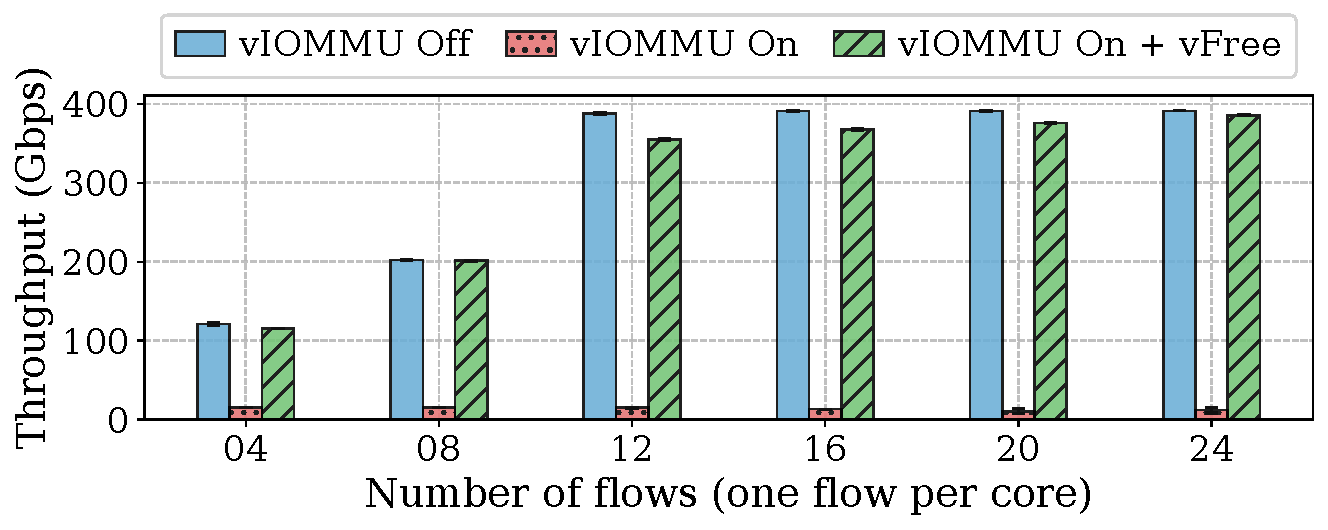
\includegraphics[width=\textwidth]{figures/tx-ebpf-tput.pdf}
        \caption{Throughput}
        \label{fig:tx-tput}
    \end{subfigure}
    \hfill
    \begin{subfigure}[b]{0.32\textwidth}
        \centering
        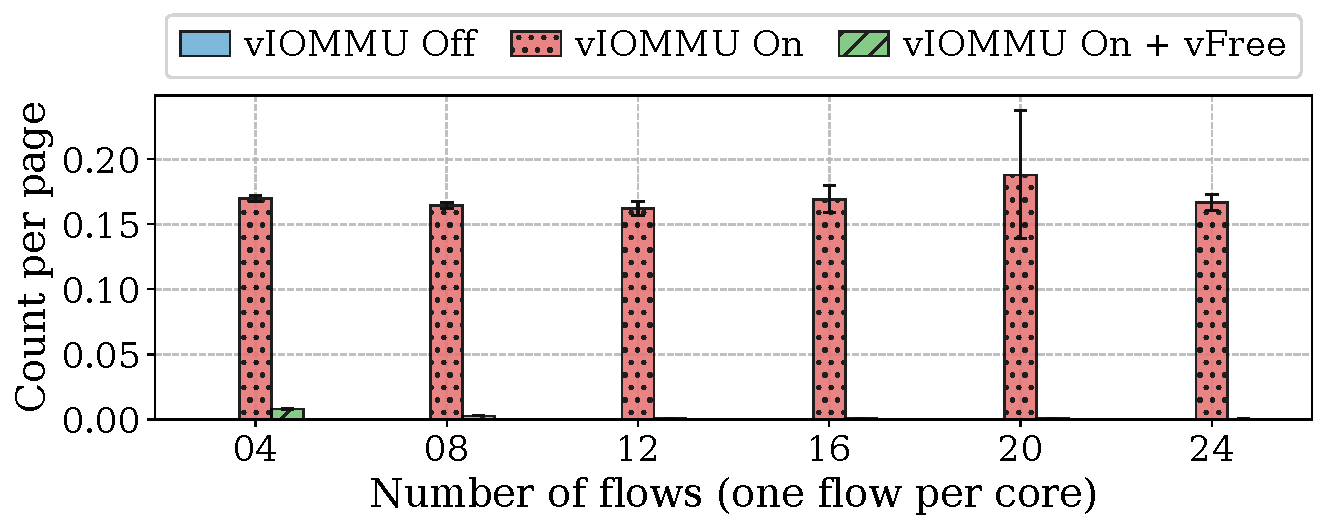
\includegraphics[width=\textwidth]{figures/tx-ebpf-qi_submit_sync-count_per_page.pdf}
        \caption{IOTLB invalidation count per page}
        \label{fig:tx-qi}
    \end{subfigure}
    \hfill
    \begin{subfigure}[b]{0.32\textwidth}
        \centering
        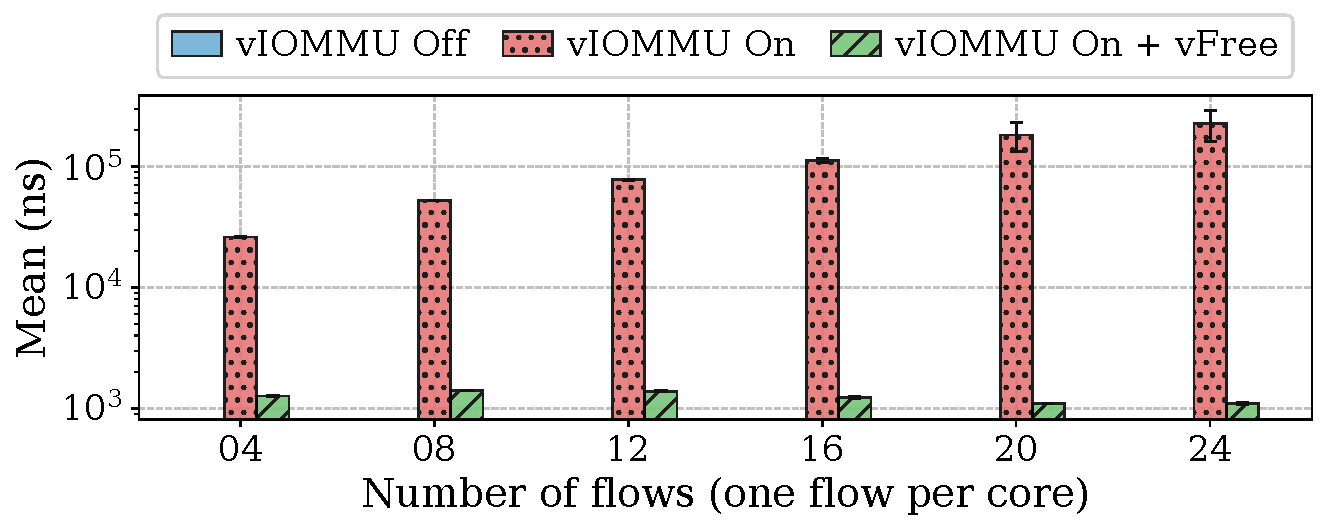
\includegraphics[width=\textwidth]{figures/tx-ebpf-cache_tag_flush_range-mean_ns.pdf}
        \caption{Average time for IOTLB invalidation}
        \label{fig:tx-flush}
    \end{subfigure} 
    \caption{Tx traffic performance of \brand.
    \todo{@Siyuan @Ishvik Fix performance plots.}
    }
    \label{fig:tx}
\end{figure*}

\newpage
\subsection{Real-world Application Performance}
We evaluate the benefits of \brand using three real-world applications: Redis \cite{redis}, nginx \cite{nginx}, and SPDK \cite{spdk}. Redis is a widely used in-memory key-value store, nginx is a widely deployed open-source web server, and SPDK is a high-performance userspace storage stack that can leverage the Linux TCP stack for remote or disaggregated storage.

For all experiments, we use the same client-server setup described in \S\ref{sec:setup}. The applications run inside the VM, while the corresponding clients run on a separate server. To approach the 400 Gbps link bandwidth, we use 24 cores and a 9K MTU size. Across these applications, we cover both Rx and Tx datapaths, as well as a mixed workload scenario.

\textbf{Redis.} With Redis, we evaluate the Rx datapath. We run 24 Redis server instances inside the VM, with one instance per core. The client machine uses the redis-benchmark utility to launch an equal number of clients, each sending \texttt{SET} requests to a corresponding server instance. We vary the \texttt{SET} value size from 8 KB to 256 KB. For each value size, we tune the number of parallel connections, client threads, and request batch size to the optimal values, and report the aggregate application throughput.

Figure \ref{fig:redis}

<\todo{@Ishvik analyze plots once results final}>

\textbf{nginx.} Using nginx, we focus on the Tx datapath. We run a single nginx server instance inside the VM \footnote{The nginx server automatically scales to handle multiple clients by spawning worker threads.}. On the client machine, we launch 24 clients, with one client pinned to each core. The clients use the \texttt{wrk} benchmark \cite{wrk} to issue HTTP \texttt{GET} requests. We vary the size of the requested web page from 128 KB to 2 MB and report the resulting aggregate throughput.

Figure \ref{fig:nginx}

<\todo{@Ishvik analyze plots once results final}>

\textbf{SPDK.} We use SPDK to evaluate a mixed read/write workload. To configure SPDK, we first create a "malloc" block device (backed by RAM) to serve read and write requests over TCP. We then run 24 SPDK server instances inside the VM, with one instance pinned to each core. The client machine runs an equal number of \texttt{fio} \cite{fio} clients, each generating a workload with 60\% reads and 40\% writes \footnote{We use a 60\% read and 40\% write workload to avoid a memory bandwidth bottleneck. Writes consume twice the memory bandwidth of reads because each write involves a memory read followed by a memory write.} at an I/O depth of 8. We vary the block size from 16 KB to 512 KB and report the aggregate throughput across reads and writes.

Figure \ref{fig:spdk}

<\todo{@Ishvik analyze plots once results final}>

\begin{figure*}[t]
    \centering
    \begin{subfigure}[b]{0.32\textwidth}
        \centering
        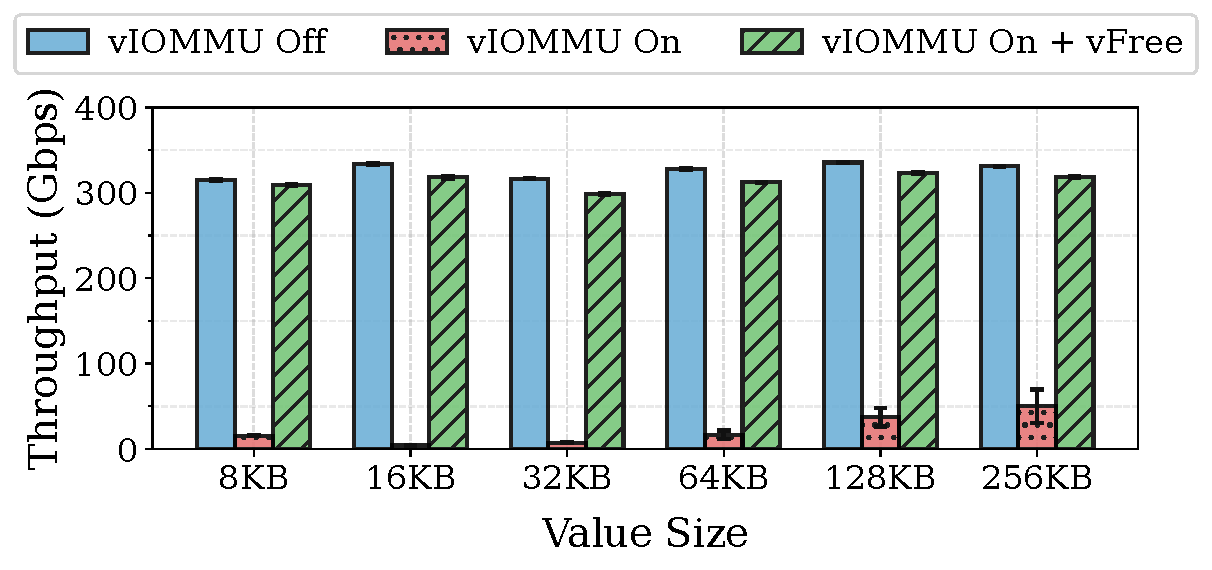
\includegraphics[width=\textwidth]{figures/redis_value_sweep.pdf}
        \caption{Redis}
        \label{fig:redis}
    \end{subfigure}
    \hfill
    \begin{subfigure}[b]{0.32\textwidth}
        \centering
        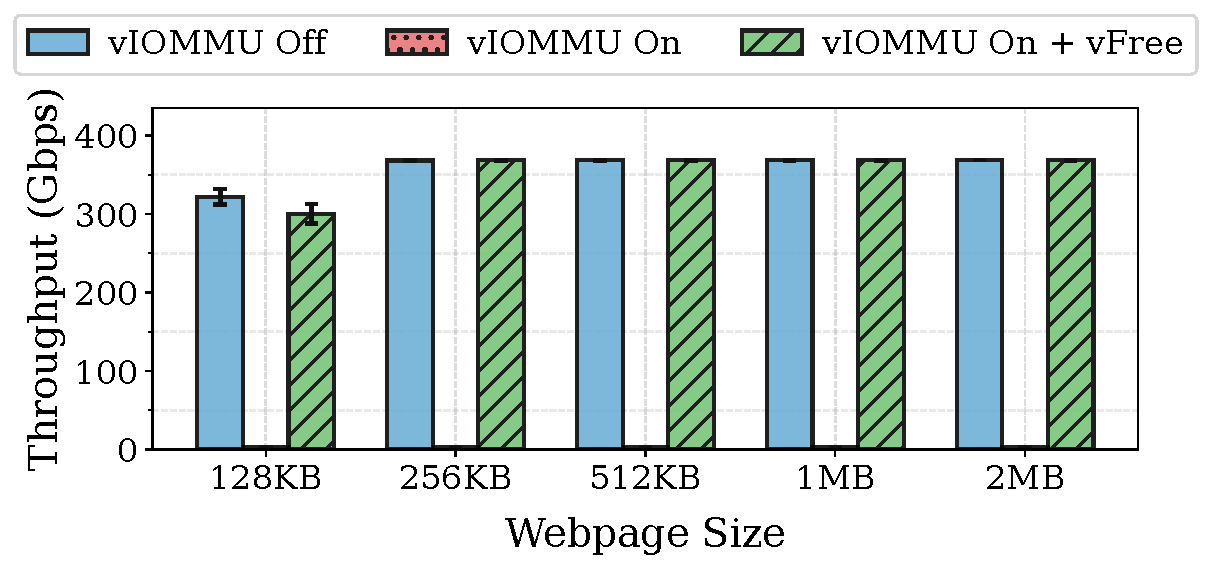
\includegraphics[width=\textwidth]{figures/nginx_size_sweep.pdf}
        \caption{nginx}
        \label{fig:nginx}
    \end{subfigure}
    \hfill
    \begin{subfigure}[b]{0.32\textwidth}
        \centering
        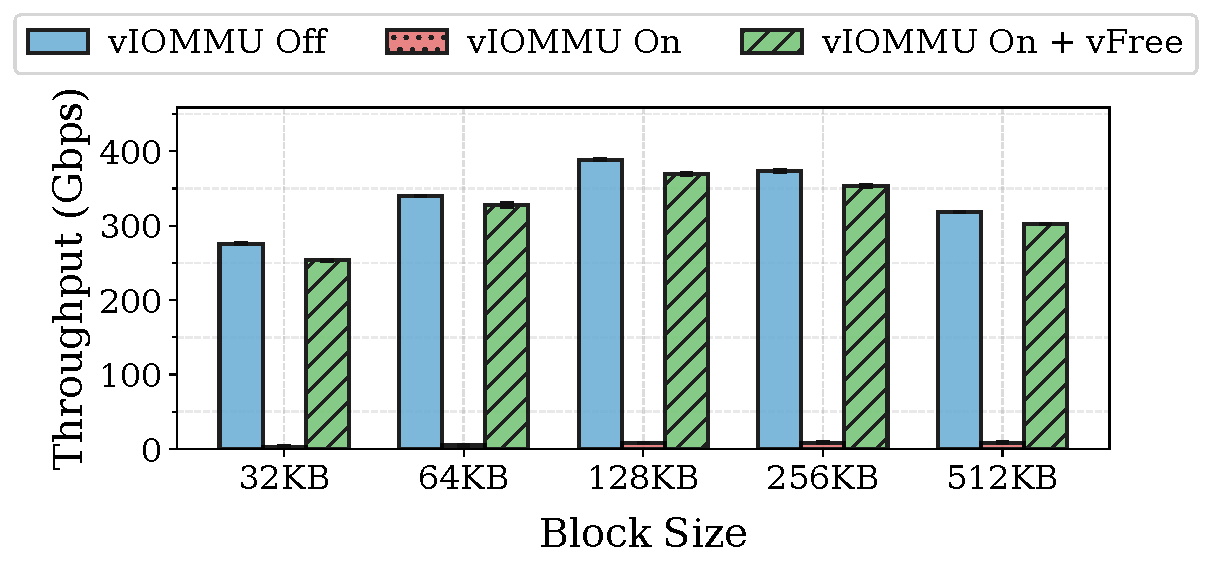
\includegraphics[width=\textwidth]{figures/spdk_fio_block_sizes.pdf}
        \caption{SPDK}
        \label{fig:spdk}
    \end{subfigure}
    \caption{Performance of real-world applications.}
    \label{fig:apps}
\end{figure*}

\subsection{Ablation Study}
\lable{sec:eval-ablation}

\begin{figure}[t]
    \centering
    % \begin{subfigure}[b]{\columnwidth}
    %     \centering
    %     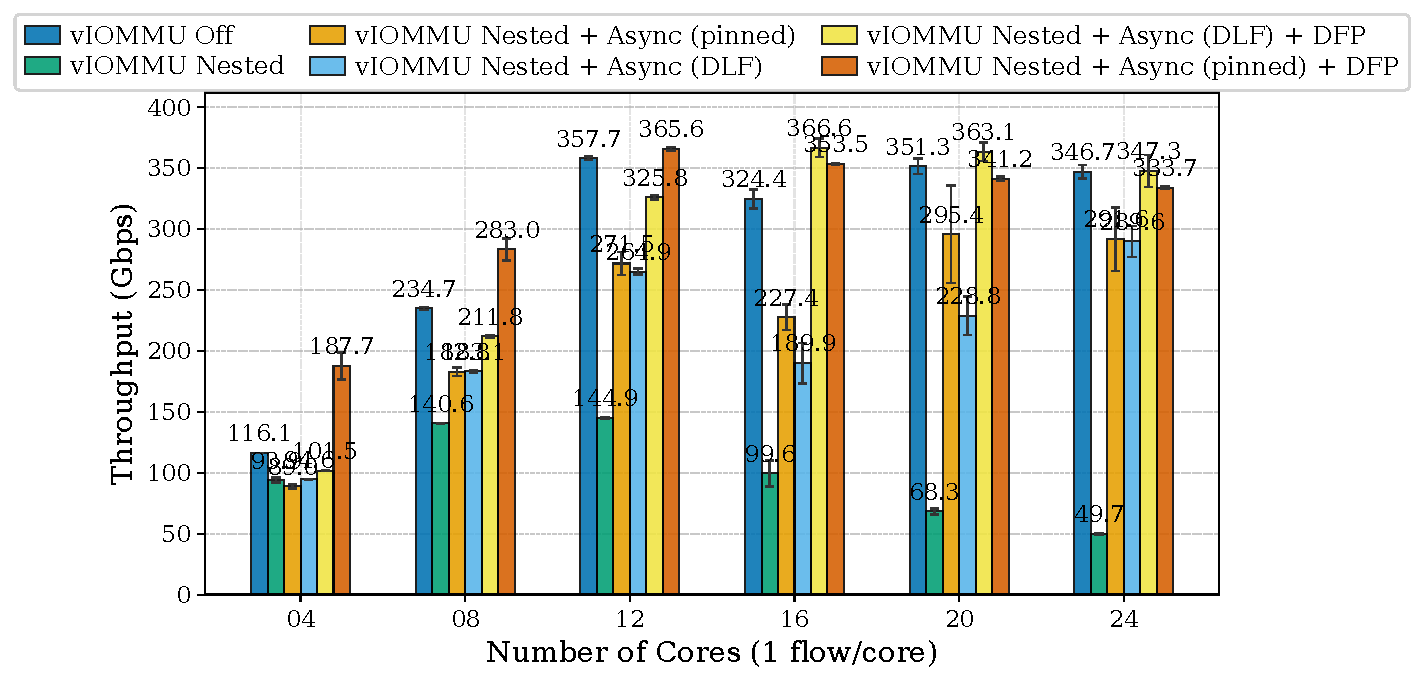
\includegraphics[width=\textwidth]{figures/eval_ablation_core_exp-tput.pdf}
    %     \caption{Ablation Study 1}
    %     \label{fig:ablation-1}
    % \end{subfigure}
    % \vspace{1em} % Add some vertical space between subfigures
    \begin{subfigure}[b]{\columnwidth}
        \centering
        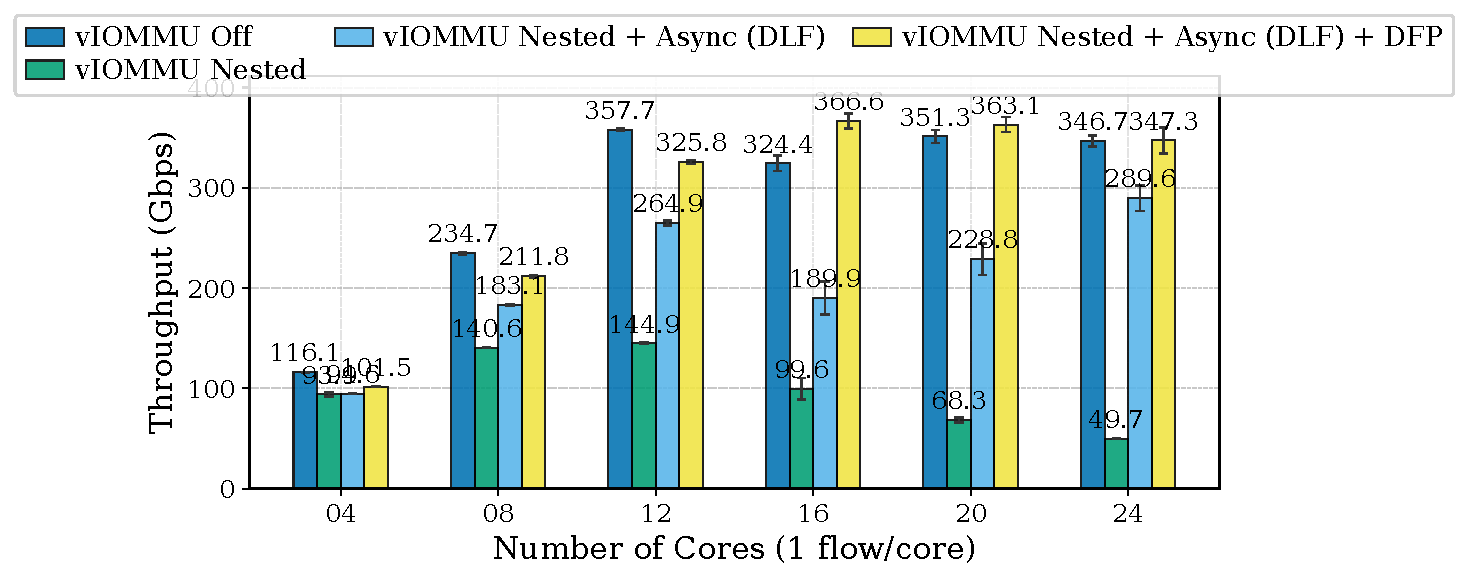
\includegraphics[width=\textwidth]{figures/eval_ablation_core_exp-tput-v2.pdf}
        \caption{Ablation Study 2}
        \label{fig:ablation-2}
    \end{subfigure}
    \caption{Ablation study results.\todo{Need Tx}}
    % \question{We only need one here. Shall we include pinned version?}}
    \label{fig:ablation}
\end{figure}

Figure \ref{fig:ablation} shows the ablation study results.

% \begin{figure}[!htbp]
%     \centering
%     \begin{subfigure}[b]{\columnwidth}
%         \centering
%         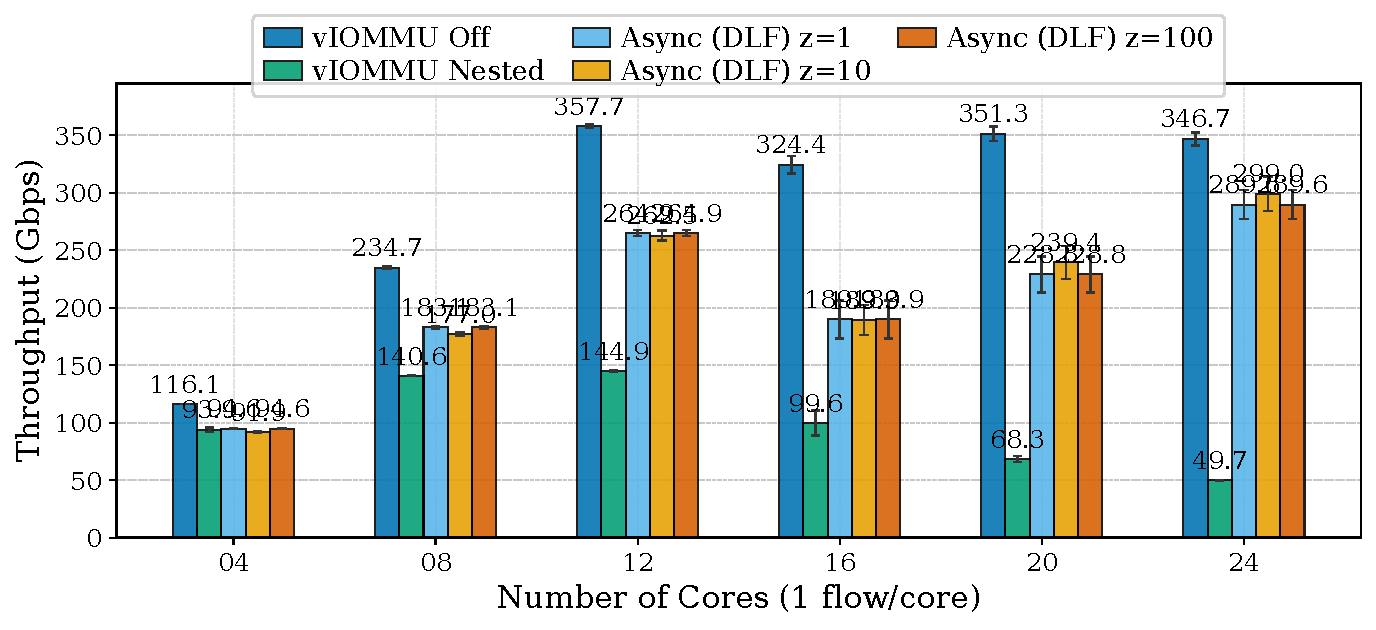
\includegraphics[width=\textwidth]{figures/eval_sensitivity_core_exp-tput.pdf}
%         \Description{Bar chart showing throughput sensitivity analysis when only Async Invalidation is enabled.}
%         \caption{Sensitivity Analysis when only Async Invalidation are enabled }
%         \label{fig:sensitivity-core}
%     \end{subfigure}
%     \vspace{1em}
%     \begin{subfigure}[b]{\columnwidth}
%         \centering
%         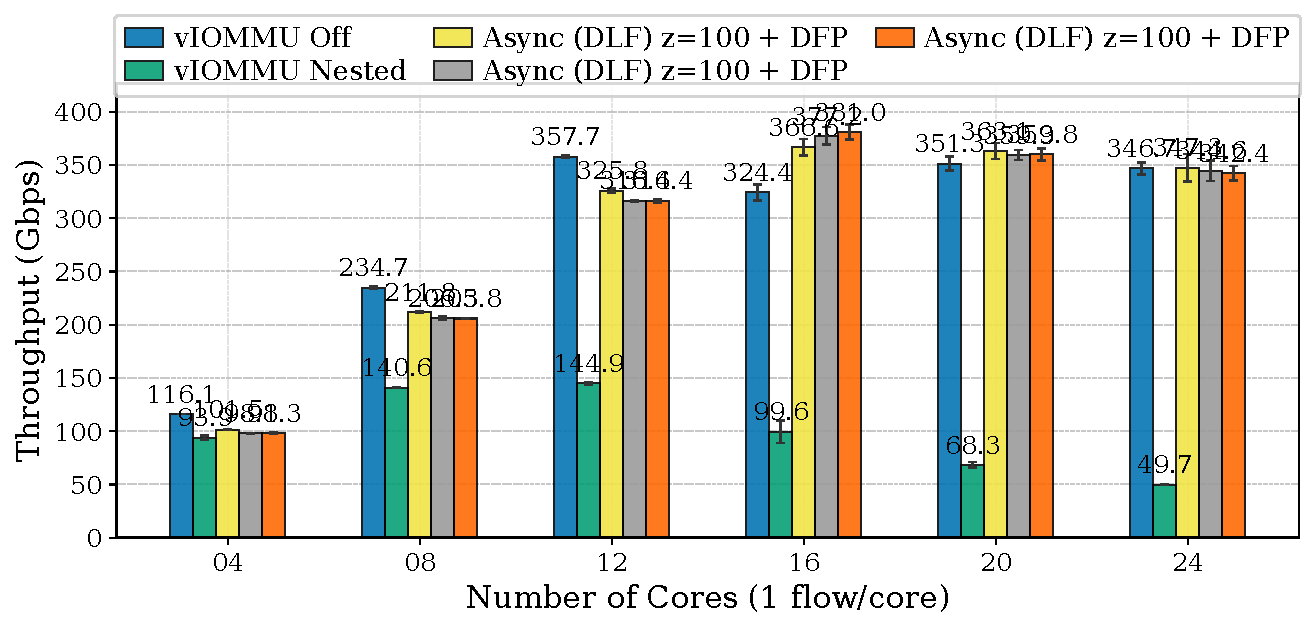
\includegraphics[width=\textwidth]{figures/eval_sensitivity_core_exp_dlf-tput.pdf}
%         \Description{Bar chart showing throughput sensitivity analysis when Async Invalidation is used with DFP.}
%         \caption{Sensitivity Analysis when only Async Invalidation is used in combination with DFP}
%         \label{fig:sensitivity-dlf}
%     \end{subfigure}
%     \caption{Parameter sensitivity of async invalidation implemented in distributed-leader-follower scheme.
%     Tested on with different maximum flushes per round (z=1, 10, 100)
    
%     \label{fig:sensitivity}
% \end{figure}

\begin{figure}[!htbp]
    \centering
    \begin{subfigure}[b]{0.49\columnwidth}
        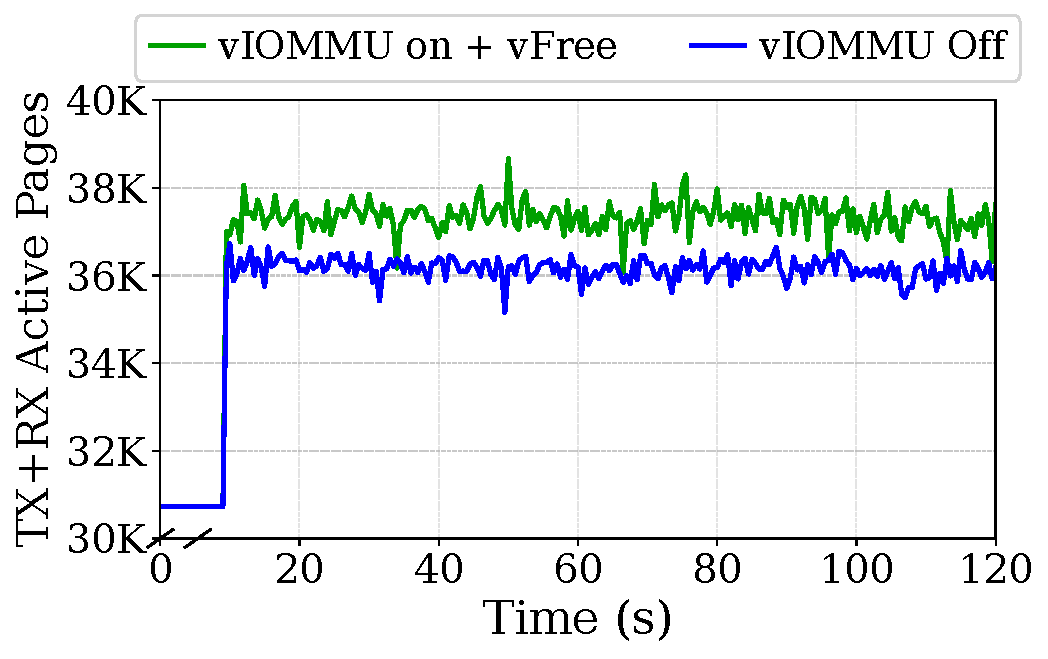
\includegraphics[width=\columnwidth]{figures/mem_fig_tx_rx_active_pages.pdf}
        \Description{Plot showing page usage over time for RX+TX case.}
        \caption{Total pages required for both RX+TX operations.}
        \label{fig:memory_total}
    \end{subfigure}
    \begin{subfigure}[b]{0.49\columnwidth}
        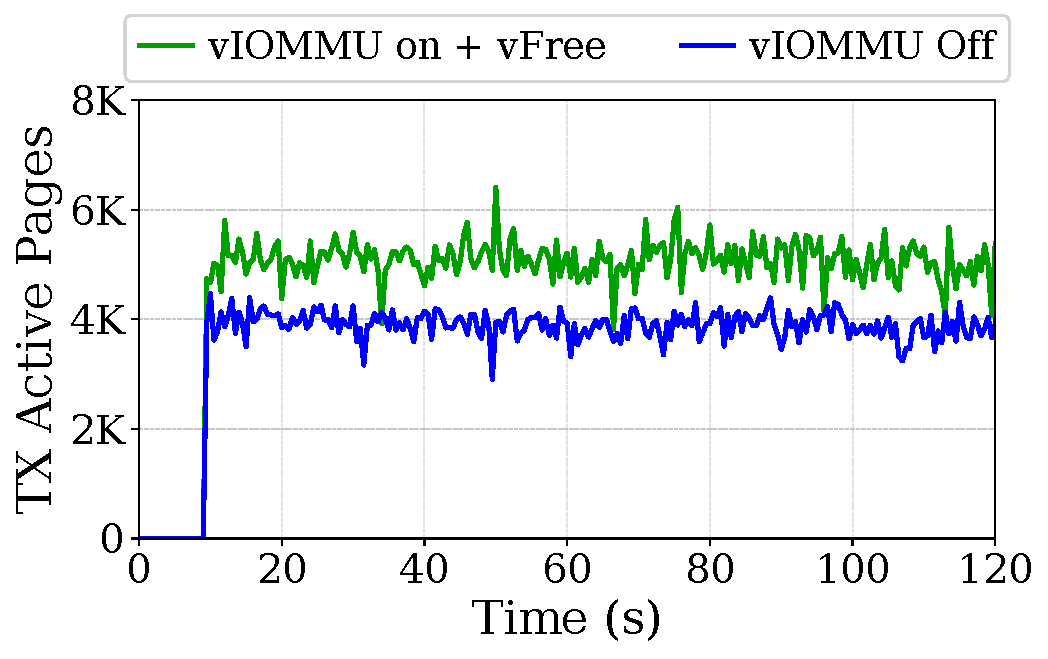
\includegraphics[width=\columnwidth]{figures/mem_fig_tx_active_pages.pdf}
        \Description{Plot showing page usage over time for TX case.}
        \caption{Total pages required for TX operations.}
        \label{fig:memory_overhead}
    \end{subfigure}
    \caption{Memory consumption comparison, note the memory overhead for TX is minimal compared to the total memory required for RX. \todo{@Owen add your data.}}
    \label{fig:rx_memory}
\end{figure}

\subsection{System Analysis}

\todo{If we have time}
\textbf{Comparison with DLF vs. pinned mode}

\todo{If we have time}
\textbf{Pinned mode on full core utilization.}
- Pinned mode: single-VM N core in total, N flows. 

\textbf{Parameter sensitivity of async invalidation.}


Figure \ref{fig:sensitivity} shows the parameter sensitivity of async invalidation implemented in distributed-leader-follower scheme.
We test with different maximum flushes per round (z=1, 10, 100).
Regardless of whether DFP is enabled, \brand's performance is not sensitive to the number of maximum flushes per round.

\textbf{Memory overhead of DFP.}

The number of pages required by the NIC driver was collected and recorded in the case where the VM is a receiver with 24 cores, with 1 flow per core. Every half second, we record the number of pages currently in use by the driver, allowing us to see the usage over the course of the execution. We find that the page requirements in the TX case can vary depending on which method is utilized \ref{fig:memory_overhead}. However, compared to the pages required in the RX case, this overhead becomes less relevant \ref{fig:memory_total}.

\clearpage


